\documentclass[a4paper,12pt]{article}

\usepackage{geometry}
\usepackage{graphicx}
\usepackage{amsmath}
\usepackage{booktabs}
\usepackage{array}
\usepackage{float}
\usepackage{hyperref}
\usepackage{xcolor}
\usepackage{listings}
\usepackage{caption}
\usepackage{enumitem}
\usepackage{xeCJK}
\usepackage{fontspec}

\geometry{left=2.5cm,right=2.5cm,top=2.6cm,bottom=2.6cm}
\hypersetup{colorlinks=true,linkcolor=black,urlcolor=blue,citecolor=black}
\setlist[itemize]{leftmargin=2em}
\setlist[enumerate]{leftmargin=2em}
\renewcommand{\arraystretch}{1.25}
\setlength{\emergencystretch}{3em}
\setmainfont{Times New Roman}
\setCJKmainfont{SimSun}
\sloppy

\lstset{
  basicstyle=\ttfamily\small,
  breaklines=true,
  frame=single,
  columns=fullflexible,
  keepspaces=true,
  backgroundcolor=\color{gray!6}
}

\title{CSE5023 Assignment 2 Report\\\large Transformer Architecture and Applications in Translation, Sentiment Analysis, and Vision}
\author{Weiqiang Duan\\Student ID: 12533582}
\date{May 17, 2026}

\begin{document}
\maketitle

\begin{abstract}
This report presents the implementation and experimental analysis for CSE5023 Assignment 2. Part 1 implements an English-to-Chinese Transformer from scratch and evaluates baseline training, cosine warm-up learning-rate tuning, architecture ablation, and positional embedding variants. Part 2 reuses the machine-translation encoder for Tweet Sentiment Extraction classification and studies the effect of removing positional embeddings. Part 3 implements a Vision Transformer on CIFAR-10 and compares it with an ImageNet-pretrained ResNet50 loaded using the PyTorch Hub interface specified in the assignment. The results show that cosine warm-up improves translation BLEU, the translation encoder transfers usefully to sentiment classification, and the pretrained CNN achieves stronger CIFAR-10 accuracy than the from-scratch ViT under the current training budget.
\end{abstract}

\tableofcontents
\newpage

\section{Part 1: English-to-Chinese Machine Translation}

This part follows the assignment structure from 1.1 to 1.5. It covers the Transformer implementation, baseline training and BLEU evaluation, cosine warm-up learning-rate tuning, architecture ablation, and positional embedding comparison. The machine-translation code is stored under \path|code/part1_machine_translation/|, and the experiment outputs are stored under \path|outputs/part1_machine_translation/|.

\subsection{Transformer Architecture}

The implementation mainly completes two files:
\begin{lstlisting}
code/part1_machine_translation/tokenization.py
code/part1_machine_translation/model/transformer.py
\end{lstlisting}

In \texttt{tokenization.py}, the \texttt{wordToID} function converts English and Chinese token sequences into integer ids. Tokens not found in the vocabulary are mapped to \texttt{UNK}. After conversion, samples are sorted by English sequence length, which reduces unnecessary padding within mini-batches.

The batch construction is handled by \texttt{MaskBatch}. The encoder input is stored in \texttt{src}, and \texttt{src\_mask} is generated by checking whether each source token is not a padding token. On the decoder side, the target sequence is shifted into \texttt{tgt[:, :-1]} as decoder input and \texttt{tgt[:, 1:]} as prediction labels. The decoder mask combines a padding mask and a causal mask, so that the decoder cannot attend to padding positions or future tokens.

In \texttt{model/transformer.py}, I implemented the feed-forward block as a two-layer MLP with ReLU and dropout, following the standard Transformer design. I also completed scaled dot-product attention in \texttt{MultiHeadAttentionBlock.attention}: attention scores are computed by query-key dot products, scaled by $\sqrt{d_k}$, masked before softmax when necessary, and finally used to aggregate value vectors.

The final \texttt{build\_transformer} function connects source/target embeddings, sinusoidal positional encodings, stacked encoder and decoder blocks, and the projection layer. This gives a complete encoder-decoder Transformer for English-to-Chinese sequence generation.

\subsubsection{Encoder and Decoder}

The encoder receives the complete English source sentence. Each encoder block contains self-attention and a feed-forward network. Since the whole source sentence is available, encoder self-attention can attend bidirectionally to all non-padding source tokens.

The decoder predicts Chinese tokens autoregressively. Each decoder block contains masked self-attention, cross-attention, and a feed-forward network. Masked self-attention only allows each target position to attend to itself and previous target positions. Cross-attention uses decoder hidden states as queries and encoder outputs as keys and values, allowing the decoder to retrieve relevant source-side information.

\subsubsection{Attention Masks}

The encoder uses a padding mask with shape \texttt{[B, 1, 1, src\_len]} to prevent attention from assigning probability mass to padded source positions. The decoder uses both a padding mask and a causal mask. The causal mask is lower-triangular, ensuring that token $t$ cannot see tokens after position $t$ during training. This is essential because the decoder must learn the same left-to-right generation process used at inference time.

\subsubsection{Training and Inference}

During training, teacher forcing is used: the ground-truth target sequence is shifted right and fed into the decoder. This allows all target positions to be processed in parallel while the causal mask preserves autoregressive constraints. During inference, the true target sentence is unavailable. The model starts from \texttt{BOS}, predicts one token at a time, appends the predicted token to the decoder input, and stops when \texttt{EOS} or the maximum length is reached.

\subsection{Training and BLEU Evaluation}

The baseline training script is:
\begin{lstlisting}
code/part1_machine_translation/translator_en2cn_baseline.py
code/part1_machine_translation/chinese_bleu.ipynb
\end{lstlisting}

The baseline model uses a 6-layer encoder and decoder, 8 attention heads, $d_{model}=256$, $d_{ff}=1024$, dropout 0.1, batch size 64, fixed learning rate $1\times10^{-4}$, and 20 training epochs. The dataset sizes are 14533 train pairs, 1817 validation pairs, and 1817 test pairs. Checkpoints are saved every 5 epochs, and validation BLEU is computed with greedy decoding.

\begin{table}[H]
\centering
\caption{Baseline Transformer Training and BLEU Results}
\label{tab:baseline-record-en}
\begin{tabular}{lr}
\toprule
Metric & Value \\
\midrule
Epochs & 20 \\
Batch size & 64 \\
Learning rate & $1\times10^{-4}$ \\
Final train loss & 1.4847 \\
Best validation BLEU & 0.1698 \\
Test BLEU & 0.1579 \\
\bottomrule
\end{tabular}
\end{table}

\begin{figure}[H]
\centering
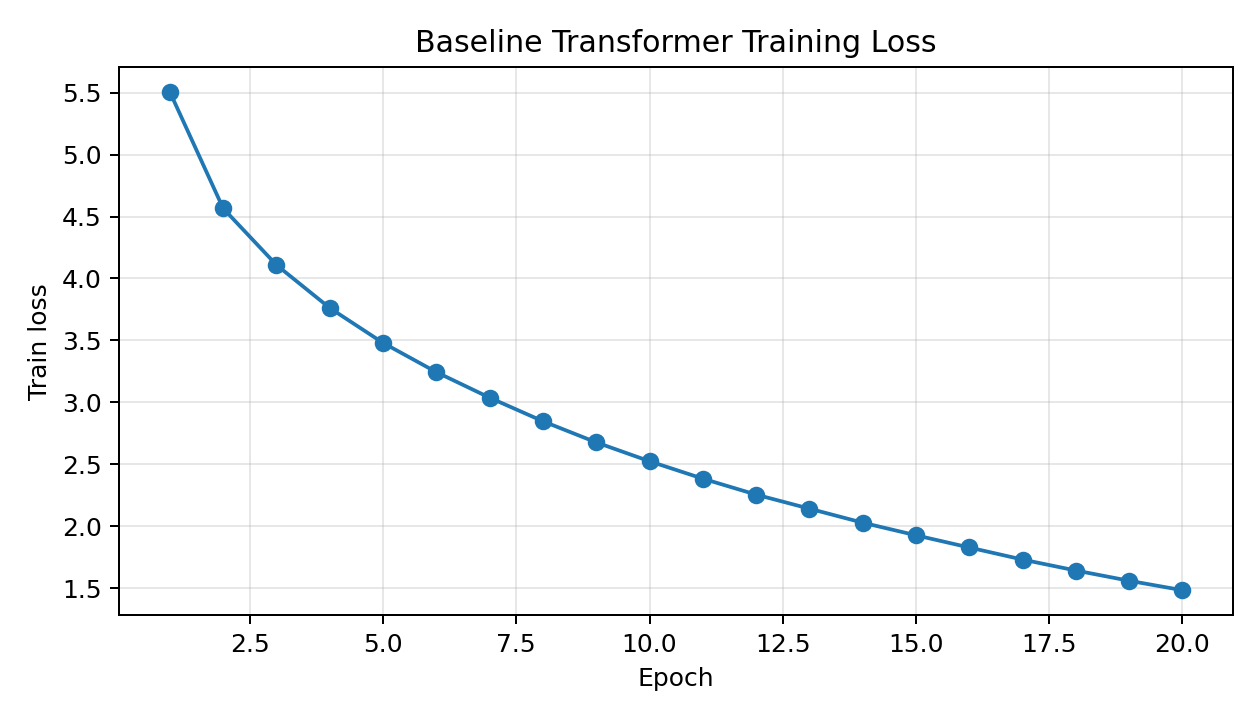
\includegraphics[width=0.72\textwidth]{../outputs/part1_machine_translation/baseline_default_6_layer/baseline_loss_curve.png}
\caption{Baseline Transformer training loss curve}
\label{fig:baseline-loss-en}
\end{figure}

For Chinese BLEU evaluation, both reference translations and model outputs are segmented with \texttt{jieba} before computing corpus BLEU. This avoids treating an entire Chinese sentence as a single token.

\begin{table}[H]
\centering
\caption{Baseline Test Translation Examples}
\label{tab:baseline-examples-en}
\begin{tabular}{p{0.22\textwidth}p{0.23\textwidth}p{0.23\textwidth}p{0.22\textwidth}}
\toprule
English input & Reference & Model output & Analysis \\
\midrule
UNK ! & 干杯! & 转！ & Unknown tokens make it difficult to recover the intended meaning. \\
listen . & 听着。 & 听听。 & The verb meaning is partly captured, but repetition appears. \\
try it . & 试试吧。 & 试试试。 & Semantically close, but the output repeats. \\
no way ! & 不可能！ & 不要！ & Negation is captured, but the exact phrase is wrong. \\
drive safely . & 安全地驾驶。 & 安静。 & The model confuses a related Chinese word and misses the driving action. \\
\bottomrule
\end{tabular}
\end{table}

The examples show that the baseline already learns some short-sentence semantics, but it still struggles with low-frequency words, repetition, and word-sense disambiguation.

\subsection{Cosine Warm-up Learning Rate Tuning}

I added cosine annealing with warm-up in \path|code/part1_machine_translation/translator_en2cn_cosine.py|. The warm-up stage linearly increases the learning rate to a peak value, and the cosine stage gradually decays it to a small minimum learning rate. All runs use the same model structure and data split; only the peak learning rate changes.

\begin{table}[H]
\centering
\caption{Cosine Warm-up Experiments with Different Peak Learning Rates}
\label{tab:cosine-en}
\begin{tabular}{lrrrr}
\toprule
Run & Final loss & Valid BLEU & Test BLEU & Best epoch \\
\midrule
peak1e-4 & 2.3193 & 0.1014 & 0.0947 & 20 \\
peak2e-4 & 1.3627 & 0.1824 & 0.1708 & 20 \\
peak3e-4 & 0.8725 & 0.2171 & 0.1999 & 20 \\
peak4e-4 & 0.5912 & 0.2344 & 0.2193 & 20 \\
peak5e-4 & 0.4302 & 0.2445 & 0.2270 & 20 \\
peak6e-4 & 0.3315 & 0.2460 & 0.2293 & 20 \\
peak7e-4 & 0.2735 & 0.2486 & 0.2339 & 20 \\
peak8e-4 & 0.2341 & 0.2550 & 0.2309 & 20 \\
\bottomrule
\end{tabular}
\end{table}

Compared with the fixed-learning-rate baseline test BLEU of 0.1579, the best test BLEU improves to 0.2339. Validation BLEU is highest with \texttt{peak\_lr=8e-4}, while test BLEU is highest with \texttt{peak\_lr=7e-4}. I therefore use \texttt{peak\_lr=7e-4} for later experiments because it gives the strongest test-set generalization.

\subsection{Transformer Architecture Ablation}

The ablation experiments use \texttt{peak\_lr=7e-4}, \texttt{warmup=5}, and \texttt{min\_lr=1e-6}. The baseline is the default 6-layer Transformer with 8 heads, $d_{model}=256$, and $d_{ff}=1024$. Each ablation changes only one architectural factor.

\begin{table}[H]
\centering
\caption{Transformer Architecture Ablation Results}
\label{tab:ablation-en}
\begin{tabular}{lrrrrrrr}
\toprule
Run & Layers & Heads & $d_{model}$ & $d_{ff}$ & Loss & Valid BLEU & Test BLEU \\
\midrule
default & 6 & 8 & 256 & 1024 & 0.2735 & 0.2486 & 0.2339 \\
nlayer3 & 3 & 8 & 256 & 1024 & 0.2800 & 0.2465 & 0.2259 \\
heads4 & 6 & 4 & 256 & 1024 & 0.3064 & 0.2432 & 0.2351 \\
dmodel128 & 6 & 8 & 128 & 512 & 1.0450 & 0.2055 & 0.1852 \\
\bottomrule
\end{tabular}
\end{table}

Reducing the number of layers only slightly increases training loss, but it reduces test BLEU. Reducing the number of heads has a small effect; the validation BLEU decreases slightly, while the test BLEU is similar. The most severe degradation comes from reducing the hidden size from 256 to 128, which hurts both convergence and BLEU. This suggests that model width is especially important for this translation setup.

\subsection{Positional Embedding}

I implemented learnable positional embedding and added a \texttt{pe\_type} option to switch between fixed sinusoidal positional encoding and learnable positional embedding. The sinusoidal baseline reuses the \texttt{cosine\_default\_6\_layer\_peak7e-4} result.

\begin{table}[H]
\centering
\caption{Sinusoidal vs. Learnable Positional Embedding}
\label{tab:position-embedding-en}
\begin{tabular}{lrrrr}
\toprule
Setting & Final loss & Valid BLEU & Test BLEU & Best epoch \\
\midrule
Sinusoidal PE & 0.2735 & 0.2486 & 0.2339 & 20 \\
Learnable PE & 0.2559 & 0.2343 & 0.2229 & 20 \\
\bottomrule
\end{tabular}
\end{table}

Learnable PE obtains a lower training loss, but its validation and test BLEU scores are lower than those of sinusoidal PE. This suggests that learnable position parameters fit the training data better but generalize less reliably under the current data scale. Sinusoidal PE provides a stable positional prior and is therefore preferred for the downstream encoder checkpoint.

\section{Part 2: Tweet Sentiment Analysis}

This part reuses the encoder from the machine-translation Transformer and fine-tunes it for three-class tweet sentiment classification. The dataset is \texttt{mteb/tweet\_sentiment\_extraction}, stored locally as JSONL files with fields \texttt{id}, \texttt{text}, \texttt{label}, and \texttt{label\_text}.

\subsection{Fine-tuning the Translation Encoder}

The selected checkpoint is:
\begin{lstlisting}
outputs/part1_machine_translation/cosine_default_6_layer_peak7e-4/best_model.pt
\end{lstlisting}

The decoder and projection layer are removed. The source embedding, source positional encoding, and encoder are reused. Tweet text is tokenized using the English vocabulary from Part 1, padded to a fixed sequence length, encoded by the Transformer encoder, pooled with mean pooling over non-padding positions, and passed to a linear classification head. Cross-entropy loss is used.

\begin{table}[H]
\centering
\caption{Tweet Sentiment Data Split}
\label{tab:sentiment-data-en}
\begin{tabular}{lr}
\toprule
Split & Samples \\
\midrule
Train & 21984 \\
Validation & 2748 \\
Test & 2749 \\
\bottomrule
\end{tabular}
\end{table}

\begin{table}[H]
\centering
\caption{Sentiment Fine-tuning Configuration}
\label{tab:sentiment-config-en}
\begin{tabular}{lr}
\toprule
Item & Value \\
\midrule
Checkpoint & \texttt{cosine\_default\_6\_layer\_peak7e-4} \\
Encoder layers & 6 \\
Hidden size & 256 \\
Attention heads & 8 \\
Pooling & mean pooling \\
Batch size & 64 \\
Epochs & 8 \\
Learning rate & $2\times10^{-4}$ \\
Weight decay & 0.01 \\
Loss & CrossEntropyLoss \\
\bottomrule
\end{tabular}
\end{table}

\begin{figure}[H]
\centering

\includegraphics[width=0.72\textwidth]{../outputs/part2_sentiment_analysis/sentiment_baseline/loss_curve.png}
\caption{Sentiment training and validation loss curves}
\label{fig:sentiment-loss-en}
\end{figure}

\begin{figure}[H]
\centering
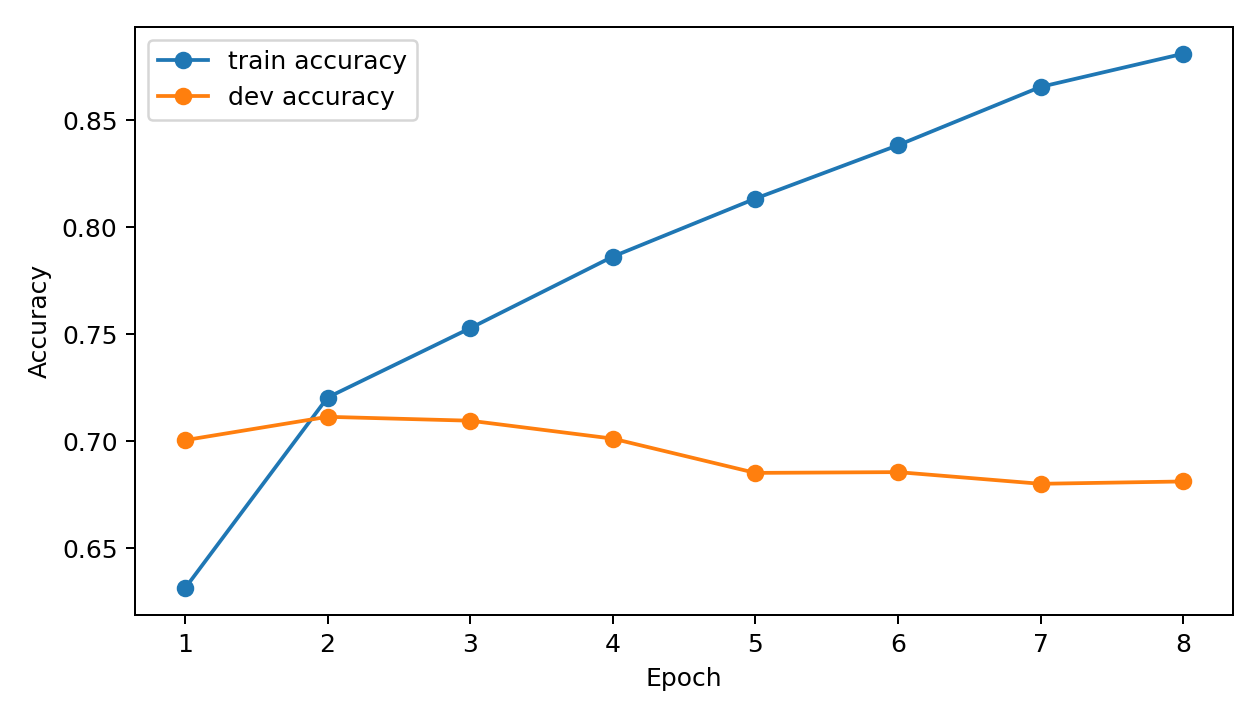
\includegraphics[width=0.72\textwidth]{../outputs/part2_sentiment_analysis/sentiment_baseline/accuracy_curve.png}
\caption{Sentiment training and validation accuracy curves}
\label{fig:sentiment-acc-en}
\end{figure}

The model reaches the best validation accuracy at epoch 2. After that, training loss continues to decrease, but validation loss increases, indicating overfitting. The epoch-2 checkpoint is therefore used for final testing.

\begin{table}[H]
\centering
\caption{Sentiment Test Results by Class}
\label{tab:sentiment-class-test-en}
\begin{tabular}{lrrrr}
\toprule
Class & Precision & Recall & F1 & Support \\
\midrule
negative & 0.6725 & 0.7416 & 0.7054 & 778 \\
neutral & 0.6851 & 0.6475 & 0.6657 & 1112 \\
positive & 0.7786 & 0.7614 & 0.7699 & 859 \\
\bottomrule
\end{tabular}
\end{table}

\begin{table}[H]
\centering
\caption{Overall Sentiment Test Results}
\label{tab:sentiment-overall-test-en}
\begin{tabular}{lr}
\toprule
Metric & Value \\
\midrule
Accuracy & 0.7097 \\
Macro Precision & 0.7120 \\
Macro Recall & 0.7168 \\
Macro F1 & 0.7137 \\
Weighted Precision & 0.7107 \\
Weighted Recall & 0.7097 \\
Weighted F1 & 0.7095 \\
Test samples & 2749 \\
\bottomrule
\end{tabular}
\end{table}

The positive class achieves the best F1 score, while the neutral class is more difficult because its boundary with mildly positive or negative tweets is less clear.

\subsection{Effect of Positional Embedding}

To study the role of positional embedding in sentiment classification, I compare the baseline with positional embedding against a version where positional embedding is removed. All other settings are kept the same.

\begin{table}[H]
\centering
\caption{Sentiment Classification With and Without Positional Embedding}
\label{tab:sentiment-pe-overall-en}
\begin{tabular}{lrrrrr}
\toprule
Setting & Best epoch & Dev acc & Test loss & Test acc & Macro F1 \\
\midrule
with PE & 2 & 0.7114 & 0.6854 & 0.7097 & 0.7137 \\
without PE & 3 & 0.7060 & 0.7058 & 0.7148 & 0.7167 \\
\bottomrule
\end{tabular}
\end{table}

\begin{table}[H]
\centering
\caption{Class-wise F1 Comparison With and Without PE}
\label{tab:sentiment-pe-class-en}
\begin{tabular}{lrr}
\toprule
Class & with PE F1 & without PE F1 \\
\midrule
negative & 0.7054 & 0.6964 \\
neutral & 0.6657 & 0.6933 \\
positive & 0.7699 & 0.7605 \\
\bottomrule
\end{tabular}
\end{table}

Removing positional embedding slightly lowers validation accuracy but slightly improves test accuracy and macro F1. The differences are small, so the main conclusion is that positional embedding is not the decisive factor for this short-text sentiment task. Unlike machine translation, which relies strongly on order, alignment, and syntax, tweet sentiment classification often depends more on sentiment-bearing words and phrases. Mean pooling further reduces the importance of exact token positions.

\section{Part 3: Vision Transformer and ResNet Comparison}

This part implements image classification on CIFAR-10. The original 50000 training images are stratified into 45000 training and 5000 validation images. The official 10000 CIFAR-10 test images are used for final evaluation.

\subsection{Vision Transformer on CIFAR-10}

The ViT code is stored in:
\begin{lstlisting}
code/part3_vision_transformer/vit_model.py
code/part3_vision_transformer/train_vit.py
\end{lstlisting}

Each $32\times32$ image is split into $4\times4$ patches, giving $8\times8=64$ patches. A convolution with kernel size and stride 4 implements patch embedding. A learnable class token and learnable positional embedding are added before the sequence is passed to a Transformer encoder. The class-token output is fed to a linear classifier.

\begin{table}[H]
\centering
\caption{ViT CIFAR-10 Configuration and Results}
\label{tab:vit-config-result-en}
\begin{tabular}{lr}
\toprule
Item & Value \\
\midrule
Patch size & 4 \\
Number of patches & 64 \\
Hidden size & 192 \\
Transformer layers & 6 \\
Attention heads & 6 \\
MLP hidden size & 384 \\
Train / Validation / Test & 45000 / 5000 / 10000 \\
Epochs & 20 \\
Best epoch & 19 \\
Best validation accuracy & 0.7364 \\
Test accuracy & 0.7276 \\
Test loss & 0.7711 \\
Parameters & 1.81M \\
Training time & 777.8 s \\
\bottomrule
\end{tabular}
\end{table}

\begin{figure}[H]
\centering

\includegraphics[width=0.72\textwidth]{../outputs/part3_vision_transformer/vit_cifar10/loss_curve.png}
\caption{ViT loss curve on CIFAR-10}
\label{fig:vit-loss-en}
\end{figure}

\begin{figure}[H]
\centering

\includegraphics[width=0.72\textwidth]{../outputs/part3_vision_transformer/vit_cifar10/accuracy_curve.png}
\caption{ViT accuracy curve on CIFAR-10}
\label{fig:vit-acc-en}
\end{figure}

The ViT training loss decreases from 1.7945 to 0.7349, and validation accuracy reaches 0.7364 at epoch 19. The final test accuracy is 0.7276.

\subsection{Comparison with a Pretrained CNN}

Following the assignment requirement, I use an ImageNet-pretrained ResNet50 as the CNN baseline. The loading code follows the provided reference:
\begin{lstlisting}[language=Python]
torch.hub.load("pytorch/vision:v0.10.0", "resnet50", pretrained=True)
\end{lstlisting}

The original 1000-class classification head is replaced with a 10-class linear layer for CIFAR-10. Since the model is pretrained on ImageNet images of size $224\times224$, CIFAR-10 images are resized to $224\times224$ and normalized using ImageNet mean and standard deviation. The ResNet50 backbone is frozen, and only the new classification head is trained.

\begin{table}[H]
\centering
\caption{ViT vs. Pretrained ResNet50 on CIFAR-10}
\label{tab:vit-resnet-compare-en}
\begin{tabular}{lrrrrr}
\toprule
Model & Epochs & Trainable params & Best val acc & Test acc & Time(s) \\
\midrule
ViT & 20 & 1.81M & 0.7364 & 0.7276 & 777.8 \\
Pretrained ResNet50 & 10 & 0.02M & 0.8286 & 0.8212 & 1560.0 \\
\bottomrule
\end{tabular}
\end{table}

\begin{figure}[H]
\centering

\includegraphics[width=0.72\textwidth]{../outputs/part3_vision_transformer/resnet50_cifar10/loss_curve.png}
\caption{Pretrained ResNet50 loss curve on CIFAR-10}
\label{fig:resnet-loss-en}
\end{figure}

\begin{figure}[H]
\centering

\includegraphics[width=0.72\textwidth]{../outputs/part3_vision_transformer/resnet50_cifar10/accuracy_curve.png}
\caption{Pretrained ResNet50 accuracy curve on CIFAR-10}
\label{fig:resnet-acc-en}
\end{figure}

The pretrained ResNet50 reaches a test accuracy of 0.8212, higher than the from-scratch ViT result of 0.7276. This comparison is not a perfectly fair architecture-only comparison because ResNet50 benefits from ImageNet pretraining while ViT is trained from scratch. However, it directly satisfies the assignment requirement and demonstrates the practical advantage of pretrained CNN features on small image datasets. CNNs also have strong local inductive biases, such as locality and translation equivariance, which are helpful for CIFAR-10. ViT is more flexible in global patch interaction, but it usually benefits from larger datasets or pretraining.

\section{Conclusion}

This assignment implements and analyzes Transformer-based models across translation, sentiment analysis, and vision tasks. In machine translation, cosine warm-up substantially improves BLEU over the fixed-learning-rate baseline, model width is important for performance, and sinusoidal positional encoding generalizes better than learnable positional embedding under the current data scale. In sentiment analysis, the translation encoder transfers useful representations, but positional embedding has only a small effect because tweet sentiment is more dependent on lexical sentiment cues. In image classification, the pretrained ResNet50 outperforms the from-scratch ViT on CIFAR-10, showing the benefit of ImageNet pretraining and CNN inductive biases for small image datasets.

\end{document}
